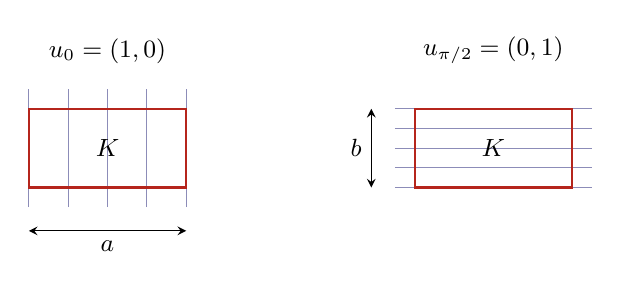
\begin{tikzpicture}[x=1cm,y=1cm,font=\small,>=stealth]
\begin{scope}
\foreach \p in {0,.5,1,1.5,2} {\draw[MidnightBlue!50] (\p,-.25)--(\p,1.25);}
\draw[BrickRed,thick] (0,0) rectangle (2,1);
\draw[<->] (0,-.55)--node[below] {$a$}(2,-.55);
\node[above] at (1,1.45) {$u_0=(1,0)$};
\node at (1,.5) {$K$};
\end{scope}
\begin{scope}[shift={(4.9,0)}]
\foreach \p in {0,.25,.5,.75,1} {\draw[MidnightBlue!50] (-.25,\p)--(2.25,\p);}
\draw[BrickRed,thick] (0,0) rectangle (2,1);
\draw[<->] (-.55,0)--node[left] {$b$}(-.55,1);
\node[above] at (1,1.45) {$u_{\pi/2}=(0,1)$};
\node at (1,.5) {$K$};
\end{scope}
\end{tikzpicture}
